\section{Techniques for planar graphs}\label{techniques}
In this section, we describe techniques popularly used in algorithms for planar graphs.

\subsection{Separators in planar graphs}
A \textit{Jordan curve} is a simple closed curve in the plane. Given a planar graph $G$,
a Jordan curve separator is a curve that intersects $G$ only at vertices. In 1984, Miller
\cite{miller1984finding} showed that for any planar graph with $n$ vertices, there is a Jordan curve
separator of size $O(\sqrt{n})$ such that each new component contains at most $2n/3$
vertices. He further showed that such a separator can be found in $O(n)$ time. \\
Frederickson introduced the \textit{$r$-division} for planar
graphs. Given an $r\in (0,n)$, the division is a decomposition of the graph into
$O(n/r)$ edge-induced subgraphs (\textit{pieces}), where each piece contains $O(r)$ vertices and $O(\sqrt{r})$ \textit{boundary vertices}. A
boundary vertex is a vertex that belongs to multiple pieces. Frederickson showed that
such a division exists for any planar graphs and can be found in $O(n\lg n)$ time. This
was achieved by applying the separator theorem of Lipton and Tarjan
\cite{lipton1979separator}, which states that for any planar graphs, there is a separator
of size $O(\sqrt{n})$ that splits $G$ into two graph each containing at most $2n/3$ of
the vertices. This was further developed
by Klein et al. \cite{klein2013structured}, who gave a $O(n)$ time algorithm to compute
an $r$-division of a planar graph $G$ with the additional property that each piece has a
constant number of \textit{holes}, which are faces of a piece that are not faces of $G$.
\\
The $r$-division we will talk about in this thesis is the one with a constant number of
holes that uses Jordan curves as separators and be computed in linear time. An
illustration of of it is shown in Figure \ref{rdiv}.

\begin{figure}[h!]
  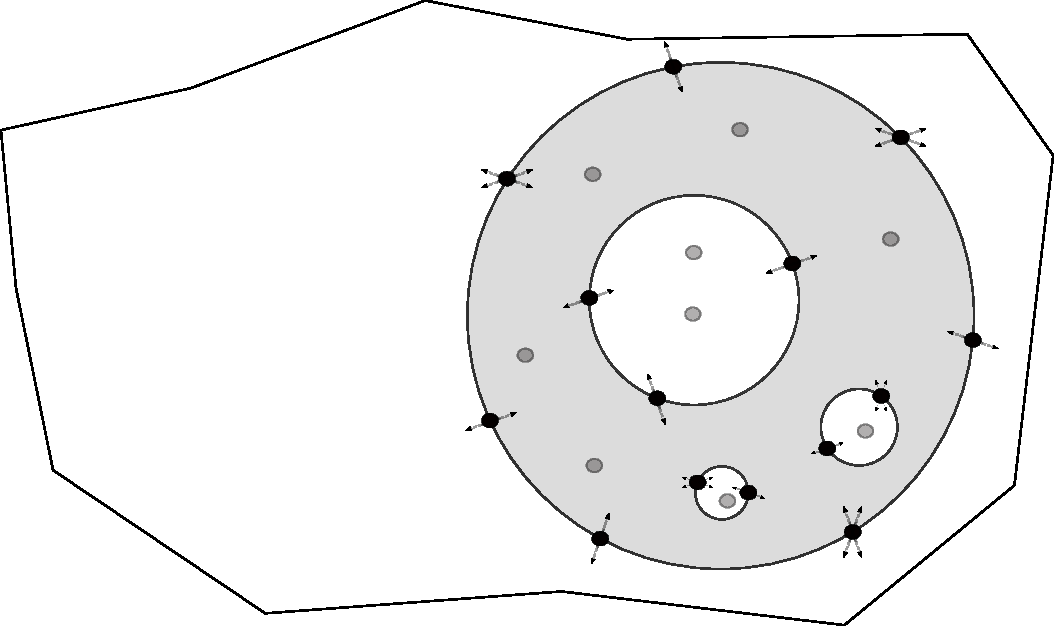
\includegraphics[width=1.0\textwidth]{figs/rdiv.pdf}
  \caption{Illustration of an $r$-division. A region $R$ of the graph $G$ is shown in
  grey with holes in white. Boundary vertices are shown as black circles, interior vertices are shown in
grey. Any edge passing through the Jordan curve goes through a boundary vertex as
indicated by the arrows.}
    \label{rdiv}
\end{figure}

\subsection{Monge property}
Given two ordered sets $A$ and $B$ and a distance function $d$, we say $d$ has the
\textit{Monge property} if for elements $u, v\in A$ and $x, y\in B$, where
$u\leq v$ and $x\leq y$, then:
\begin{align*}
  d(u,x)+d(v,y)\leq d(u, y)+d(v,x)
\end{align*}
An example of this is shortest paths distances between boundary vertices in planar graph
given all four boundary vertices lie on the infinite face. It states that the sum of
paths that do not cross is at most the sum of paths that do cross. Figure \ref{monge}
illustrates this. \\
Another implication of the property is that if we have found the $u$ that minimizes $d(u,y)$,
then for all boundary vertices $v$ that are on  counter clockwise path on the face $f$
(according to Figure \ref{monge}), then $d(v,x)\geq d(u,x)$. To see this, note that there
is a vertex $w$ on path from $u$ to $y$ that the path $v$ to $x$ must cross. Since
$d(u,y)\leq d(v,y)$, it implies that $d(u,w)\leq d(v,w)$. It is important that all
vertices are on the boundary of the face as it is otherwise not true (as indicated by
Figure \ref{monge2}). \\
The \textit{Monge matching problem} is finding the parent $p(v)\in A$ for all $v\in B$,
so that $d(p(v), v)\leq d(u,v)$ for any $u\in A$. The \textit{minimum Monge matching} is
the set of $(p(v), v)$.

\begin{figure}
  \centering
  \begin{subfigure}[b]{0.45\textwidth}
    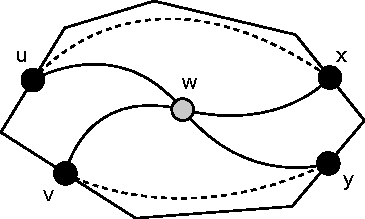
\includegraphics[width=\textwidth]{figs/monge.pdf}
    \caption{Illustration of the Monge property in planar graphs. The sum of the distances
  when paths cross (in solid) are less than or equal to the sum of distances when paths
do not cross (in dashed lines).}
    \label{monge}
  \end{subfigure}
  \quad
  \begin{subfigure}[b]{0.45\textwidth}
    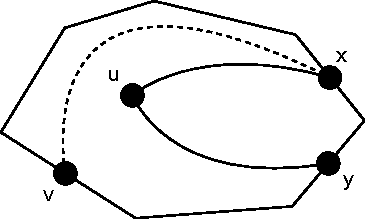
\includegraphics[width=\textwidth]{figs/monge2.pdf}
    \caption{A scenario where the Monge property does not hold, since paths
      do not cross. The shortest paths from $u$ are
      indicated by solid lines and a shorter path to $x$ is indicated by a dashed line.}
    \label{monge2}
  \end{subfigure}
\end{figure}

\subsection{Klein's multiple source shortest path}
Klein's multiple source shortest path \cite{klein2005multiple} is another useful tool for planar
graphs. Given a planar graph with nonnegative weight, we can construct a data structure
of size $O(n \lg n)$ that can answer queries of the following form in $O(\lg n)$ time:
For a source vertex $v$ and a vertex $s$ on the boundary of the infinite face, find the
shortest path from $v$ to $s$. This is especially useful to compute all pairs shortest paths between boundary
nodes in an $r$-division as it requires $O(r\lg r)$ time for a region $R$. \\
The idea is then to compute a shortest path tree $T$ rooted at
$s_i$ and then modifying the tree to get the shortest path tree rooted at the
neighbouring boundary vertex $s_{i+1}$. Using an efficient representation of dynamic
trees that allow operations to be done in amortized $O(\lg n)$ time is possible
\cite{tarjan2005self}\cite{henzinger1999randomized}. Any edge will then join the tree at
most once and leave the tree at most once. Since the graph is planar, we have $O(r)$ edges,
giving us the $O(r\lg r)$ running time. \\
The query idea is to use an Euler tour representation of the tree, called $T$, so we can
return the distance from a vertex $u$ to the root $r$ of the tree. Since we need the
correct version of the tree computed during preprocessing, we need a persistent data
structure that remembers changes, so we can recover any state of $T$.

\begin{figure}[h!]
  \centering
  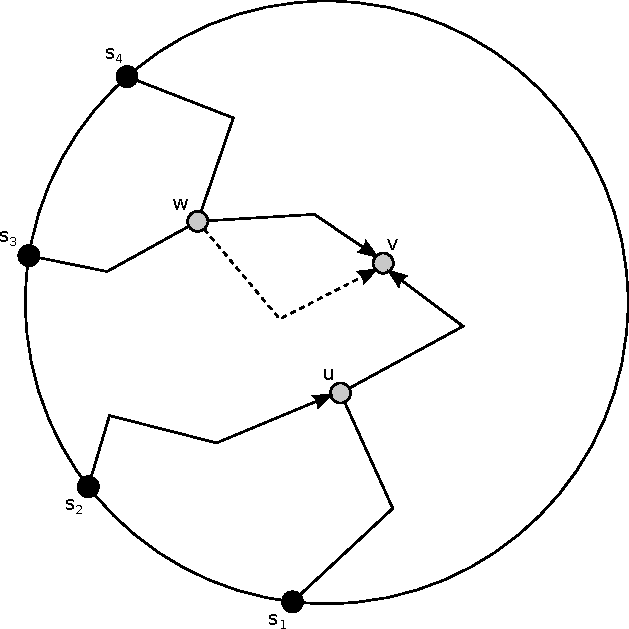
\includegraphics[width=0.6\textwidth]{figs/klein.pdf}
  \caption{Illustration of Klein's MSSP structure. The idea is two adjacent boundary
    vertices have almost identical shortest path trees. Computing shortest path trees
    $T_i$ clockwise
    around the face from $s_1$, we need only consider the \textit{differences} between
  the two trees. The dashed line is an impossible situation. Having computed the shortest
path tree rooted in $s_3$, $T_3$, where the shortest path to $v$ goes through $w$, it is
impossible for the shortest path tree rooted in $s_4$ to "cross" $T_3$ since it would
imply a shorter path from $w$ to $v$.}
    \label{klein}
\end{figure}

\subsection{FR-Djikstra}
A \textit{dense distance graph} or DDG is defined over a decomposition of a planar
graph. It is the non-planar graph $G'$ of $G$ where there is an edge $uv$ if both $u$ and
$v$ are boundary nodes with weight equal to the shortest path between the vertices.
Fakcharoenphol and Rao \cite{fakcharoenphol2006planar} gave an algorithm that can answer
distance queries between nodes in $O(\sqrt{n}\lg^2 n)$ after $O(n\lg^3 n)$ preprocessing.
The decomposition used in the algorithm is the result of applying a separator
recursively. For each level, the graph is split into "inside" and "outside" of the
separator. They then compute and store a MSSP for both inside and outside. At the same
time, we obtain the shortest paths between boundary nodes in the graph. Using Klein's
algorithm \cite{klein2005shortest}, this can be done in $O(n\lg n)$ time for each level.
The depth of the recursion is $O(\lg n)$, which means we can get preprocessing down to
$O(n\lg^2 n)$ time using $O(n\lg n)$ space. \\
After consutrcting the dense distance graph, it is possible to to compute a shortest path
tree $T$ in $G'$ that obey the Monge property. Using the Monge property, they can compute
$T$ in time linear to number of vertices in $G'$ which is significantly lower than the
number of vertices in $G$. Specifically, the graph is divided into bipartite graph that
all comply with the Monge property and then invoke a Djikstra-like algorithm that run in
time proportional to the number of vertices in $G'$.
